\documentclass[english,11pt,twoside,a4paper]{article}
\usepackage[left=2cm,top=1cm,right=2cm,nohead,nofoot]{geometry}
\usepackage[utf8]{inputenc}
\usepackage{hyperref}
\usepackage{amssymb}
\usepackage{graphicx}
\usepackage{titling}
\usepackage{listings}
\usepackage{appendix}
\newcommand{\subtitle}[1]{%
  \posttitle{%
    \par\end{center}
    \begin{center}\large#1\end{center}
    \vskip0.5em}%
}

\begin{document}
\author{
  Muona, Leo
}
\title{Mini-PL Interpreter}
\subtitle{Compilers - Project report}

\maketitle

\tableofcontents

\section{Introduction}

This document is a project report for University of Helsinki course Compilers. The subject of the project is to create an interpreter for specified Mini-PL programming language. The interpreter must scan, parse, construct an AST (abstract syntax tree) and run valid Mini-PL programs. The suggested programming language for the project was C\#, but I wrote this compiler in C++, since it is much easier to develop C++ in a Linux environment.

This report includes documentation for setup and compiling the interpreter, interpreters architectural documentation and how tokens are constructed by the scanner. Documentation also includes Mini-PL's context-free grammar used by the parser, creation of abstract syntax tree, and how errors are handled trough the program.

\section{Setup and compiling}

This Mini-PL interpreter is written in C++, in a Linux environment and has not been tested in Windows or OSX environment. Interpreter is tested in the following environment and thus have them as system requirements:

\begin{itemize}
	\item Linux operating system (kernel 3.10)
	\item GCC 4.7
	\item CMake 2.8
	\item GNU Make 3.82
\end{itemize}

It may (and probably does) also support older version of the listed software versions. In order to compile the interpreter, use the following commands in interpreters root directory:

\begin{lstlisting}[language=bash]
  $ mkdir build
  $ cd build
  $ cmake ..
  $ make
\end{lstlisting}

Now you can run the interpreter by using mpli with Mini-PL file as parameter, i.e.

\begin{lstlisting}[language=bash]
  $ ./mpli file1.mpli
\end{lstlisting}

If you want to enable debug messages, to see parse tree and AST, please modify define variable DEBUG\_MPLI to 1 in file main.cpp.

\section{Architecture}

This Mini-PL interpreter can be divided into four main components: Scanner, Parser, AST and Interpreter. Each of them have their own "jobs" and can be considered to be the four phases of the program:

\begin{itemize}
	\item Scanner: Scans character stream and constructs valid tokens that are given to the Parser.
	\item Parser: Parses the token stream into parse tree. This is used by the AST.
	\item AST: Constructs an abstract syntax tree from parse tree. This is used by the Interpreter.
	\item Interpreter: Runs the program that is described by abstract syntax tree.
\end{itemize}

If one of these components produce errors, the compiling stops and program exits without calling the next phase of the compiler.

\begin{figure}
	\begin{center}
		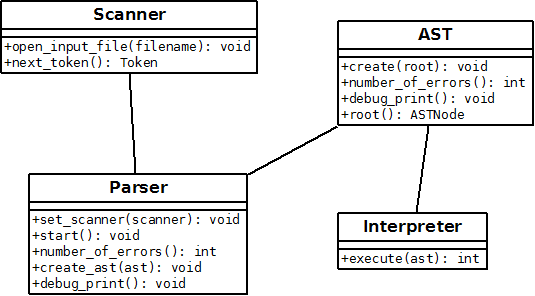
\includegraphics[scale=0.7]{class_diagram.png}
		\caption{Class diagram of the interpreter}
	\end{center}
	\label{class_diagram1}
\end{figure}

Figure~\ref{class_diagram1} shows the connections between classes, and their methods. Execution of the program goes as following:

\begin{itemize}
	\item 1. scanner.open\_input\_file(filename);
	\item 2. parser.set\_scanner(scanner);
	\item 3. parser.start();
	\item 4. parser.create\_ast(ast);
	\item 5. interpreter.execute(ast);
\end{itemize}

Parser's start()-function calls scanner's next\_token()-function as many times as there are tokens incoming. After that parser creates the AST and then interpreter executes the AST.

\section{Token construction}

Scanner creates tokens via state automaton. In Scanner's constructor, a map of state arrays are initialized that has the movement information between states. In a list below are token types as a list and how they are constructed. Some of them are not in state automaton, as token type is defined later by comparison.

\begin{itemize}
	\item IDENTIFIER: automaton: <alphabetical> ( <alpha>|<numeric>|'\_' )*
	\item INTEGER: automaton: <numeric> ( <numeric> )*
	\item STRING: automaton: '"' ( <any> )* '"'
	\item DOUBLEDOT: automaton: '.' '.'
	\item COLON: automaton: ':'
	\item INSERT: automaton: ':' '='
	\item SEMICOLON: automaton: ';'
	\item BRACKET\_RIGHT: automaton: ')'
	\item BRACKET\_LEFT: automaton: '('
	\item OP\_ADD: automaton: '+'
	\item OP\_SUBT: automaton: '-'
	\item OP\_DIVIS: automaton: '/'
	\item OP\_NOT: automaton: '!'
	\item OP\_MULT: automaton: '*'
	\item OP\_AND: automaton: '\&'
	\item OP\_LT: automaton: '<'
	\item OP\_EQ: automaton: '='
	\item KW\_VAR: check if IDENTIFIER is keyword.
	\item KW\_FOR: check if IDENTIFIER is keyword.
	\item KW\_END: check if IDENTIFIER is keyword.
	\item KW\_IN: check if IDENTIFIER is keyword.
	\item KW\_DO: check if IDENTIFIER is keyword.
	\item KW\_READ: check if IDENTIFIER is keyword.
	\item KW\_PRINT: check if IDENTIFIER is keyword.
	\item KW\_INT: check if IDENTIFIER is keyword.
	\item KW\_STRING: check if IDENTIFIER is keyword.
	\item KW\_BOOL: check if IDENTIFIER is keyword.
	\item KW\_ASSERT: check if IDENTIFIER is keyword.
	\item END\_OF\_FILE: file ended?
	\item ERROR: if token type cannot be defined.
\end{itemize}

\section{Mini-PL context-free grammar}

Parser uses the default context-free grammar that was defined by the original assignment:

\begin{lstlisting}
 <prog>   ::=  <stmts>
 <stmts>  ::=  <stmt> ";" ( <stmt> ";" )*
 <stmt>   ::=  "var" <var_ident> ":" <type> [ ":=" <expr> ] 
           |   <var_ident> ":=" <expr>  
           |   "for" <var_ident> "in" <expr> ".." <expr> "do" 
                  <stmts> "end" "for"  
           |   "read" <var_ident>  
           |   "print" <expr>  
           |   "assert" "(" <expr> ")"

 <expr>   ::=  <opnd> <op> <opnd>
           |   [ <unary_op> ] <opnd>
		   
 <opnd>   ::=  <int>
           |   <string>
           |   <var_ident>
           |   "(" expr ")"
              
 <type>   ::=  "int" | "string" | "bool"
 <var_ident> ::= <ident>
 
 <reserved keyword> ::= 
              "var" | "for" | "end" | "in" | "do" | "read" | 
              "print" | "int" | "string" | "bool" | "assert"
\end{lstlisting}

However, there are some limitations to this. <op> stands for operators '+', '-', '*', '/', '<', '=', '\&' and '!'. However integers have only following operators allowed: '+', '-', '*', '/', '<', '=' and '!'. String values have only the following operators allowed: '+', '=' and '!'. Boolean values have only '\&' and '!' allowed.

For <unary\_op> (which is '!'), only boolean value may follow it. Boolean values are produced either by '<', '=' and '!' operators or bool variables. String values can be appended with integer values by using '+' with string value as left-side operator.

There is a limitation to read statement, in which you cannot set a boolean value with read. A limitation to for statement is also applied in which you must have integer values as range. Also, analysis insists that variable used in for-in loop is defined as integer.

\section{Abstract syntax tree}

Abstract syntax tree is constructed from parse tree. This is done by removing "unnecessary" nodes and transforming other nodes into AST's node format. A list of AST node types and child node types are the following:

\begin{itemize}
	\item ROOT: possible child nodes are: INSERT, FOR\_LOOP, READ, PRINT, ASSERT and VAR\_INIT.
	\item INSERT: child nodes are in order: VAR\_ID and (OPERATOR or UNARY\_OP or VAR\_ID or CONSTANT).
	\item OPERATOR: child nodes are in order: (OPERATOR or UNARY\_OP or VAR\_ID or CONSTANT) and (OPERATOR or UNARY\_OP or VAR\_ID or CONSTANT).
	\item UNARY\_OP: child node is OPERATOR, UNARY\_OP, VAR\_ID or CONSTANT.
    \item FOR\_LOOP: child nodes are in order: FOR\_IN and FOR\_DO.
    \item FOR\_IN: child nodes are in order: VAR\_ID, (OPERATOR or VAR\_ID or CONSTANT) and (OPERATOR or VAR\_ID or CONSTANT).
    \item FOR\_DO: possible child nodes are: INSERT, FOR\_LOOP, READ, PRINT, ASSERT and VAR\_INIT.
    \item READ: child node is VAR\_ID.
    \item PRINT: child node is OPERATOR, UNARY\_OP, VAR\_ID or CONSTANT.
    \item ASSERT: child node is child node is OPERATOR, UNARY\_OP, VAR\_ID or CONSTANT.
    \item VAR\_ID: no child nodes.
    \item VAR\_INIT: child node is VAR\_ID.
    \item CONSTANT: no child nodes.
\end{itemize}

\section{Error handling}

Scanner does not handle errors. It merely just creates ERROR type tokens that it gives to Parser. Parser and AST handles errors by counting and printing them. Interpreter merely just prints errors it notices. However, certain parts of Interpreter throws std::invalid\_argument exceptions because they cannot just print and return error code, since return values from them are always "valid".

Lexical errors are identified by Scanner but printed out by Parser. Syntactical errors are identified and printed out by Parser. Semantic errors are either noticed by AST or Interpreter depending on error type. 

\section{Limitations, bugs and needed improvements}

I have noticed added the following limitation(s) to original specification:
\begin{itemize}
	\item Nested /* */ comments are not supported. C does not support them and I don't like them. However, reason them being left out was because of coding time running out.
\end{itemize}

I have noticed the following bug(s) in my interpreter:
\begin{itemize}
	\item Scanner does not notice negative integer values. This is a major bug.
	\item Scanner allows integer to start with zero. This is a major bug.
	\item Interpreter prints \\n signs in strings as characters instead of line change. This is a minor bug.
\end{itemize}

Following item(s) could be to-do improvements for the interpreter:
\begin{itemize}
	\item Better error reporting: Include line number and token that causes the error.
	\item Support for multiple input files.
	\item Use only cstdio or iostream, not both.
	\item Enhance code style and algorithms.
\end{itemize}

\newpage
\appendix
\section{\\Project specification} \label{App:ProjectSpec}

Implement an interpreter for the Mini-PL programming language. The language analyzer must correctly recognize and process all valid (and invalid) Mini-PL programs. It should report syntactic errors, and then continue analyzing the rest of the source program. It must also construct an AST and make necessary passes over this program representation. The semantic analysis part binds names to their declarations, and checks semantic constraints, e.g., expressions types and their correct use. If the given program was found free from errors, the interpreter part will immediately execute it.

\subsection{Implementation requirements and grading criteria}

The assignment is done as individual work. When building your interpreter, you are expected to properly use and apply the compiler techniques taught and discussed in the lectures and exercises. The Mini-PL analyzer is to be written purely in a general-purpose programming language. C\# is to be used as the implementation language, by default (if you have problems, please consult the teaching assistant). No special language-processing tools (language recognizer generators, regex libraries, translator frameworks, etc.) are allowed. Note that you can use the basic general data structures of the host language - such as strings and string builders, lists/arrays, and associative tables (dictionaries, maps). You must yourself make sure that your system can be run on the development tools available at the CS department.
The emphasis on one part of the grading is the quality of the implementation: especially its overall architecture, clarity, and modularity. Pay attention to programming style and commenting. Grading of the code will consider (undocumented) bugs, level of completion, and its overall success (solves the problem correctly). Try to separate the general (and potentially reusable) parts of the system (text handling and buffering, and other utilities) from the source-language dependent issues.

\subsection{Documentation}

Write a report on the assignment, as a document in PDF format. The title page of the document must show appropriate identifications: the name of the student, the name of the course, the name of the project, and the valid date and time of delivery.
Describe the overall architecture of your language processor with, e.g., UML diagrams. Explain your diagrams. Clearly describe yout testing, and the design of test data. Tell about possible shortcomings of your program (if well documented they might be partly forgiven). Give instructions how to build and run your interpreter. The report must include the following parts

The Mini-PL token patterns as regular expressions or, alternatively, as regular definitions.
A modified context-free grammar suitable for recursive-descent parsing (eliminating any LL(1) violations); modifications must not affect the language that is accepted.
Specify abstract syntax trees (AST), i.e., the internal representation for Mini-PL programs; you can use UML diagrams or alternatively give a syntax-based definition of the abstract syntax.
Error handling approach and solutions used in your Mini-PL implementation (in its scanner, parser, semantic analyzer, and interpreter).
For completeness, include the original project definition and the Mini-PL specification as appendices of your document; you can refer to them when explaining your solutions.

\subsection{Delivery of the work}

The final delivery is due at 23 o'clock (11 p.m.) on Sunday 16th of March. After the appointed deadline, the maximum points to be gained for a delivered work diminishes linearly, decreasing two (2) points per each hour late.
The work should be returned to the exercise assistant via e-mail, in a zip form. This zip (included in the e-mail message) should contain all relevant files, within a directory that is named according to your unique department user name. The deliverable zip file must contain (at least) the following subfolders.

  <username>
    ./doc
    ./src 
When naming your document (.pdf) and project (.zip) files, always include your CS user name and the packaging date. These constitute nice unique names that help to identify the files later. Names would be then something like: 
 
   document:  laster\_doc\_2013\_11\_4.pdf 
   project zip: laster\_proj\_2013\_11\_4.zip

More detailed instructions and the requirements for the assignment are given in the exercise group. If you have questions about the folder structure and the ways of delivery, or in case you have questions about the whole project or its requirements, please contact the teaching assistant (Zach Laster).

\newpage
\section{\\Mini-PL specification} \label{App:MiniPLSpec}

Mini-PL is an uncomplicated programming language designed for pedagogic purposes. The language is purposely simplified and is not meant for any real programming. Mini-PL contains few statements, arithmetic expressions, and some IO primitives. The language uses static typing and has three built-in types representing primitive values: int, string, and bool. The BNF-style syntax of Mini-PL is given below, and the following paragraphs informally describe the semantics of the language. 
 
Mini-PL uses a single global scope for all different kinds of names. All variables must declared before use, and each identifier may be declared once only. If not explicitly initialized, variables are assigned an appropriate default value. 
 
The Mini-PL read statement can read either an integer value or a whitespace-limited word (string) from the input stream. Likewise, the print statement can write out either integers or string values. A Mini-PL program uses default input and output channels defined by its environment. Additionally, Mini-PL includes an assert statement that can be used to verify assertions (assumptions) about the state of the program. An assert statement takes a bool argument. If an assertion fails (the argument is false) the system prints out a diagnostic message. The assignment statement (":=") and arithmetic expressions have their usual meanings - as in common programming languages. 
 
A for statement iterates over the consequent values from a specified integer range. The expressions specifying the beginning and end of the range are evaluated once only (at the beginning of the for statement). The for control variable behaves like a constant inside the loop: it cannot be assigned another value (before exiting the for statement). A control variable needs to be declared before its use in a for statement (in the global scope).

\subsection{Context-free grammar for Mini-PL}

The syntax definition is given in so-called Extended Backus-Naur form (EBNF). In the following Mini-PL grammar, the notation X* means 0, 1, or more repetitions of the item X. The '|' operator is used to define alternative constructs. Parentheses may be used to group together a sequence of related symbols. Brackets ("[" "]") may be used to enclose optional parts (i.e., zero or one occurrence). Reserved keywords are marked bold (as "var"). Operators, separators, and other single or multiple character tokens are enclosed within quotes (as: ".."). Note that nested expressions are always fully parenthesized to specify the execution order of operations. 
 \begin{lstlisting}
 <prog>   ::=  <stmts>
 <stmts>  ::=  <stmt> ";" ( <stmt> ";" )*
 <stmt>   ::=  "var" <var_ident> ":" <type> [ ":=" <expr> ] 
           |   <var_ident> ":=" <expr>  
           |   "for" <var_ident> "in" <expr> ".." <expr> "do" 
                  <stmts> "end" "for"  
           |   "read" <var_ident>  
           |   "print" <expr>  
           |   "assert" "(" <expr> ")"

 <expr>   ::=  <opnd> <op> <opnd>
           |   [ <unary_op> ] <opnd>
		   
 <opnd>   ::=  <int>
           |   <string>
           |   <var_ident>
           |   "(" expr ")"
              
 <type>   ::=  "int" | "string" | "bool"
 <var_ident> ::= <ident>
 
 <reserved keyword> ::= 
              "var" | "for" | "end" | "in" | "do" | "read" | 
              "print" | "int" | "string" | "bool" | "assert"
   \end{lstlisting}          
\subsection{Lexical issues}

In the syntax definition the symbol <ident> stands for an identifier token. An identifier is a sequence of letters, digits, and underscores, starting with a letter. Uppercase letters are distinguished from lowercase.
 
In the syntax definition the symbol <int> stands for an integer constant. An integer constant is a sequence of decimal digits. The symbol <string> stands for a string literal. String literals follow the C-style convention: any special characters, such as the quote character (") or backslash (\\), are represented as escape characters (e.g.: \\"). 
 
In the syntax definition the symbol <op> stands for an operator symbol. A limited set of binary operators include (only!) the ones listed below. 
 \begin{lstlisting}
'+' | '-' | '*' | '/' | '<' | '=' | & | '!'. 
 \end{lstlisting}
There is one unary operator symbol: '!', meaning the logical not operation. The operator symbol '\&' stands for the logical and operation. Note that in Mini-PL, '=' is the equal operator - not assignment. 
 
The predefined type names (e.g.,"int") are reserved keywords, so they cannot be used as (arbitrary) identifiers. In a Mini-PL program, a comment may appear between any two tokens. There are two forms of comments: one starts with "/*", ends with "*/", can extend over multiple lines, and may be nested. The other comment alternative begins with "//" and goes only to the end of the line. 


\subsection{Sample programs}
\begin{lstlisting}
     var X : int := 4 + (6 * 2);
     print X;
\end{lstlisting}
\begin{lstlisting}
     var nTimes : int := 0;
     print "How many times?"; 
     read nTimes; 
     var x : int;
     for x in 0..nTimes-1 do 
         print x;
         print " : Hello, World!\n";
     end for;
     assert (x = nTimes);
\end{lstlisting}
\begin{lstlisting}

     print "Give a number"; 
     var n : int;
     read n;
     var f : int := 1;
     var i : int;
     for i in 1..n do 
         f := f * i;
     end for;
     print "The result is: ";
     print f; 
\end{lstlisting}

\end{document}
